\newpage 
\section[Continuity]{\hyperlink{toc}{Continuity}}

\subsection{Limits and Continuity}
\begin{definition}{Limits}{4.1}
    Let $X, Y$ be metric spaces. Let $E \subset X$, and let $f: E \rightarrow Y$. Let $p \in X$ be a limit point of $E$. Then, we say that $\lim_{x\rightarrow p} f(x) = q$ or $f(x) \rightarrow q$ as $x \rightarrow p$ if there exists $q \in Y$ such that for all $e > 0$, there exists $\delta > 0$ such that for all $x \in E$ with $0 < d_X(x, p) < \delta$ we have that $d_Y(f(x), q) < \e$. 
\end{definition}
\noindent Note in the above definition that we do not care about $f(p)$, that is, the actual value of $f$ at $p$. In particular, if $p \notin E$, then $f(p)$ is not even necessarily defined. This distinction between the limit and the actual value of a function at a point becomes crucial later on when we want to define a derivative. Although we will discuss this in more detail in Chapter 5, the definition of a derivative of a function $g$ at a point $p \in \RR$ involves the function $f: \RR \rightarrow \RR$ such that:
\begin{align*}
    f(x) = \frac{g(x) - g(p)}{x - p}
\end{align*}
Evidently, the domain of $f$ does not contain the point $p$, but we are interested in the value of $f$ in the limit of $x \rightarrow p$ (which, if it exists, is the value of the derivative).

\begin{figure}[htbp]
    \centering
    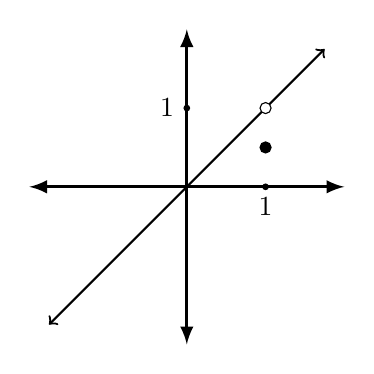
\begin{tikzpicture}
        \draw[latex-latex,very thick] (-2,0)--(2,0);
        \draw[latex-latex,very thick] (0,-2)--(0,2);
        \draw[<->, thick] (-1.75, -1.75) -- (1.75, 1.75);
        \draw[fill = black] (0, 1) circle (1pt);
        \node[xshift = -0.25cm] at (0, 1) {$1$};
        \draw[fill = black] (1, 0) circle (1pt);
        \node[yshift = -0.25cm] at (1, 0) {$1$};
        \draw[fill = white] (1, 1) circle (2pt);
        \draw[fill = black] (1, 0.5) circle (2pt);
    \end{tikzpicture}
    
    \caption{Visualization of the function $f(x) = x$ for $x \in \RR \setminus \set{1}$, $f(x) = 0$ for $x = 1$. In this case, we have that $f(1) = 0$ but $\lim_{x \rightarrow 1} f(x) = 1$, demonstrating that the actual value of the function is irrelevant when defining the limit.}
    \label{fig17}
\end{figure}

\begin{theorem}{}{4.2}
    Let $X, Y$ be metric spaces. Let $E \subset X$ and $f:E \mapsto Y$. Suppose that for all sequences $\set{p_n} \subset E$ with $p_n \rightarrow p$ and $p_n \neq p$, we have that $f(p_n) \rightarrow q \in Y$. Then, this is equivalent to saying that $\lim_{x \rightarrow p} f(x) = q$.
\end{theorem}
\begin{nproof}
    \boxed{\implies} Suppose that $\lim_{x \rightarrow p} f(x) = q$, and let $\set{p_n}$ be a sequence in $E$ with $p_n \rightarrow p$ and $p_n \neq p$ for all $n$. We wish to show that $f(p_n) \rightarrow q$. Let $\e > 0$. We show that there exists $N \in \NN$ such that $d_Y(f(p_n), q) < \e$ for all $n \geq N$. Since $\lim_{x \rightarrow p} f(x) = q$, there exists $\delta > 0$ such that for all $x \in E$ with $d_X(p, x) < \delta$, $d_Y(f(x),q) < \e$. Since we know that $p_n \rightarrow p$, there exists some $N$ such that $0 < d(p_n, p) < \delta$ for all $n \geq N$, so we have that $d_Y(f(p_n), q) < \e$ as required. 

    \boxed{\impliedby} We show the contrapositive. Suppose that $\lim_{x \rightarrow p} f(x) \neq q$. We wish to find a sequence $\set{p_n} \subset E$ with $p_n \rightarrow p$ and $p_n \neq p$ for all $n$ such that $f(p_n)$ does not converge to $q$. Since $\lim_{x \rightarrow p} f(x) \neq q$, then there exists $\e > 0$ such that for all $\delta > 0$, there exists $x \in E$ such that $0 < d_X(x, p) < \delta$ but $d_Y(f(x), q) \geq \e$. For each $\delta$ of the form $\frac{1}{n}$, let $p_n \in E$ be the corresponding value of $x$. Then, $p_n \rightarrow p$, $p_n \neq p$ for all $n$, and $f(p_n)$ does not converge to $q$ as $d(f(p_n), q) \geq \e$ for all $n$. \qed
\end{nproof}

\stepcounter{rudin}

\begin{theorem}{}{4.4}
    
\end{theorem}

\subsection{Topological Characterization of Continuity}

\subsection{Continuity and Compactness}

\subsection{Uniform Continuiity, Connectedness, and IVT}

